\chapter{El transistor MOSFET}

\section{Introducción}

\lipsum[1]

\section{Capacitor MOS}


\lipsum[1-2]

\begin{equation*}
	\phi_F \equiv \phi_B \equiv E_i(\text{sustrato}) - E_F 
    = \frac{kT}{q} \log \parentesis{\frac{N_A}{n_i}} = -\frac{kT}{q} \log \parentesis{\frac{N_D}{n_i}} 
\end{equation*}
\begin{equation*}
	\phi_S \equiv E_i(\text{sustrato}) - E_i (\text{interfaz}) 
\end{equation*}

\subsection{Capactior MOS ideal}

\lipsum[1-2]




\begin{equation*}
	\Ecal_S (x) = \left\lbrace \begin{array}{ll}
		\frac{qN_A}{K_S \epsilon_0} (W-x) & \quad \text{si} 0\leq W \leq x \\
		0 & \quad \text{si} \ W<x 
	\end{array} \right.
\end{equation*}



\begin{equation*}
	V_G = \phi_S + \frac{K_S}{K_o} x_o \sqrt{\frac{2qN_A}{K_S\epsilon_0} \phi_s}
\end{equation*}

\subsection{No idealidades}

En el MOS ideal hemos trabajado en el caso de que el concepto banda plana y equilibrio termodinámico se cumplen simultáneamente, sin embargo no son lo mismo. Decimos que nuestro MOS está en \textbf{banda plana} cuando las bandas $E_i,E_V$ y $E_c$ son constantes, aunque las bandas de Fermi del metal y semiconductor no coincidan; y que está en \textbf{equilibrio termodinámico} $V_G=0$ cuando no hay ningún voltaje aplicado, lo que implica que las bandas son iguales $E_F(\text{metal}) = E_F(\text{semiconductor})$, aunque las bandas de conducción y valencia no sean constantes (se curvan).

Hay dos puntos que afectan directamente a la forma de las bandas y el MOS. Estos son: 

\begin{itemize}
	\item La diferencia de trabajo metal-semicondcutor.
	\item Las cargas en el óxido.
\end{itemize}

\subsubsection{Diferencia de trabajo}

Cuando la diferencia de trabajo entre el metal y el semicondcutor puede hacer que aparezca un potencial $V_G$ incluso cuando no conectamos terminales de voltaje. Al valor este lo llamamos \textbf{tensión de banda plana} ya que es la tensión que tenemos que introducir nosotros para que las bandas de fermi de ambos lados sean iguales. 

Así pues, ahora distinguiremos $V_{pol}$ como el voltaje entre que nostros introducimos y $V_{FB}$ como el voltaje de puerta que tenemos cuando $V_{pol}=0$ o el voltaje $V_{pol}$ que tenemos que introducir para que $V_{G}=0$. Así tenemos que:

\begin{equation}
	V_G = - \frac{1}{q} (E_F (\text{metal}) - E_F (\text{semiconductor}) ) = V_{pol} + V_{FB}
\end{equation}
ya que definimos 
\begin{equation}
	V_{FB} = \chi_{met} - \parentesis{\chi_{sil} + \frac{1}{q} (E_c-E_i) + \frac{1}{q} (E_i-E_F)}
\end{equation}
Con las siguientes aproximaciones siempre qeu estemos en el caso de \textbf{polisilicio tipo N} o \textbf{polisilicio tipo P}: 

\begin{equation}
	\chi_{Pol. N} = \chi_{sil} \qquad  \chi_{Pol. P} = \chi_{sil} + E_g
\end{equation}

\subsubsection{Cargas en el óxido}

Aparecen diferentes cargas en toda la región del óxido y de su interfaz, provocando grandes cambios en las cruvas, dependiendo del a temperatura. El mayor problema es que crean dispositivos inestables, y podemos estudiar su efecto resolviendo las ecuaciones de Poisson teniendo en cuenta las cargas. Hay 4 tipos de centros de carga: 

\begin{itemize}
	\item Iones móviles.
	\item Carga fija. 
	\item Cargas en interfaz.
	\item Cargas inducidas. 
\end{itemize}
Los modulamos a través de la ecuación capacidad-voltaje:

\begin{equation}
	\Delta V = \frac{Q}{C}
\end{equation}
tal que $C=C_o$ y $Q$ serán las diferentes cargas del óxido. El efecto de las cargas del óxido entonces:

\begin{equation}
	V_{ox} = - \frac{Q_F}{C_0}
\end{equation}
siendo $Q_F$ las \textbf{cargas en el óxido}. 

\subsubsection{Efecto total}

El efecto total, sumando las contribuciones por diferencia de trabajo y cargas en el óxido es:

\begin{equation}
	V_{G} = V_{pol} + V_{FB} - V_{ox}
\end{equation}

\section{Transistores MOSFET}



Es un dispositivo de 4 terminales, con 2 versiones: 
\begin{itemize}
	\item Sustrato tipo P con dos regiones $N^+$ formando fuente y drenador. Se le llama \textit{MOSFET de canal n}.
	\item Sustrato tipo N con dos regiones $P^+$ formando fuente y drenador. Se le llama \textit{MOSFET de canal p}.
\end{itemize}
\begin{figure}
	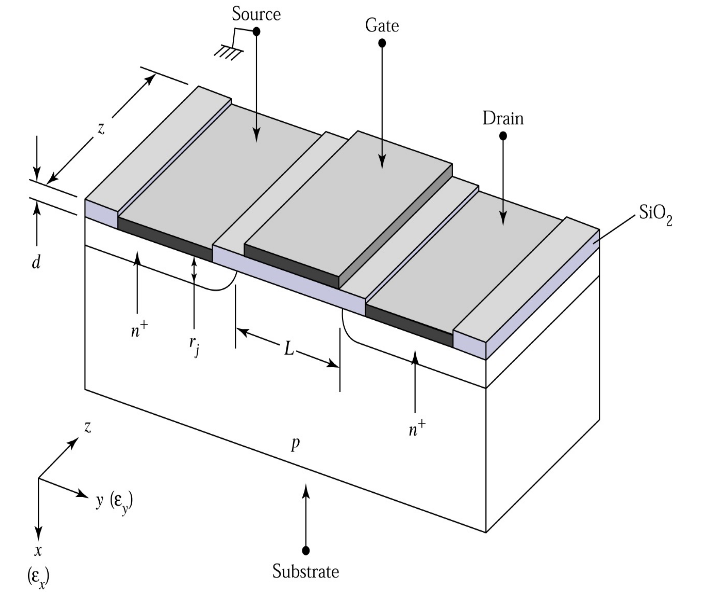
\includegraphics[width=0.6\linewidth]{Cuerpo/Ch_05/Figura-01.png}
	\caption{transistor MOSFET.}
	\label{Fig:05-01}
\end{figure}
Y los parámetros principales son longitud de canal $L$, ancho de canal $Z$, espesor de óxido $d$, profundidad de las uniones $r$ y el dopado del sustrato.

El funcionamiento del MOSFET es sencillo. El MOS se coloca en inversión tal qeu cerca del óxido aparece una región con portadores mayoritarios huecos (si el sustrato es tipo $n$) o electrones (si el sustrato es tipo $p$Z)

